\documentclass[10pt,a4paper,twocolumn,twoside]{article}
\usepackage[utf8]{inputenc}
\usepackage[catalan]{babel}
\usepackage{multicol}
\usepackage{graphicx}
\usepackage{fancyhdr}
\usepackage{times}
\usepackage{titlesec}
\usepackage{multirow}
\usepackage{lettrine}
\usepackage{xurl}
\usepackage[hidelinks]{hyperref}
\usepackage[top=2cm, bottom=1.5cm, left=2cm, right=2cm]{geometry}
\usepackage[figurename=Fig.,tablename=TAULA]{caption}
\usepackage{float}
\captionsetup[table]{textfont=sc}

\author{\LARGE\sffamily Lara Castillejo Roig}
\title{\Huge{\sffamily Sistema Automàtic de Detecció d'Errors en Gimnàstica Artística mitjançant Deep Learning}}

\newcommand\blfootnote[1]{%
  \begingroup
  \renewcommand\thefootnote{}\footnote{#1}%
  \addtocounter{footnote}{-1}%
  \endgroup
}

\titleformat{\section}
{\large\sffamily\scshape\bfseries}
{\textbf{\thesection}}{1em}{}

\begin{document}

\fancyhead[LO]{\scriptsize Lara Castillejo Roig: Sistema Automàtic de Detecció d'Errors en Gimnàstica Artística mitjançant Deep Learning}
\fancyhead[RO]{\thepage}
\fancyhead[LE]{\thepage}
\fancyhead[RE]{\scriptsize EE/UAB TFG INFORMÀTICA: Sistema Automàtic de Detecció d'Errors en Gimnàstica Artística mitjançant Deep Learning}

\fancyfoot[CO,CE]{}

\fancypagestyle{primerapagina}
{
   \fancyhf{}
   \fancyhead[L]{\scriptsize TFG EN ENGINYERIA INFORMÀTICA, ESCOLA D'ENGINYERIA (EE), UNIVERSITAT AUTÒNOMA DE BARCELONA (UAB)}
   \fancyfoot[C]{\scriptsize Maig de 2026, Escola d'Enginyeria (UAB)}
}

\renewcommand{\headrulewidth}{0pt}
\renewcommand{\footrulewidth}{0pt}
\pagestyle{fancy}

\twocolumn[\begin{@twocolumnfalse}

\maketitle

\thispagestyle{primerapagina}

\begin{center}
{\vrule depth 0pt height 0.5pt width 4cm\hspace{7.5pt}%
\raisebox{-3.5pt}{\fontfamily{pzd}\fontencoding{U}\fontseries{m}\fontshape{n}\fontsize{11}{12}\selectfont\char70}%
\hspace{7.5pt}\vrule depth 0pt height 0.5pt width 4cm\relax}
\end{center}

\end{@twocolumnfalse}]

\section{Introducció}

\lettrine[lines=3]{E}{ls} Jocs Olímpics de París 2024 van evidenciar una problemàtica històrica en la gimnàstica artística: la immensa dificultat d'arbitrar rutines d'alta velocitat de forma exclusivament manual. La polèmica mediàtica sorgida a la final de terra femenina, centrada en la validació del grau de rotació d'un salt acrobàtic per a la Nota de Dificultat (\textit{D-Score})\cite{paris_2024}, va posar de manifest la pressió i la càrrega cognitiva a la qual estan sotmesos els jutges. Si bé en la dificultat existeix una via de reclamació oficial, els jutges depenen exclusivament de la seva agudesa visual per detectar petits errors biomecànics en fraccions de segon. Aquest factor humà introdueix una inevitable subjectivitat en l'avaluació de la Nota d'Execució (\textit{E-Score}) \cite{olympics_scoring}. Aquesta nota avalua exclusivament la perfecció tècnica de l'exercici: parteix d'una base de 10.0 punts sobre la qual els jutges apliquen deduccions per cada error de postura, flexió o aterratge. Es tracta d'una puntuació crítica que, a diferència de la dificultat, és estrictament inalterable segons el reglament.

Tot i que la intel·ligència artificial ja s'utilitza a competicions Olímpiques mitjançant el sistema multimilionari d'escaneig 3D \textit{Judging Support System}, desenvolupat per \textit{Fujitsu} \cite{fujitsu_jss}, el seu elevat cost el fa inaccessible fora de l'èlit mundial. Això deixa milers de clubs de tecnificació i atletes amateurs sense eines d'anàlisi biomecànica objectives.


\section{Objectius}

L'objectiu principal d'aquest projecte és democratitzar l'accés a l'anàlisi esportiva desenvolupant un sistema automàtic de detecció d'errors basat en Visió per Computador de baix cost a partir de vídeos monoculars.

Per tal d'assolir aquesta fita principal, i garantint una anàlisi rigorosa de com els models d'intel·ligència artificial s'adapten a la complexitat de les acrobàcies d'alta velocitat, es defineixen els següents objectius específics:

\begin{enumerate}
    \item \textbf{Auditoria i Selecció de l'Arquitectura:} Avaluar comparativament l'eficiència de diferents models de \textit{Human Pose Estimation} (\textit{HPE}) (arquitectures \textit{Top-Down} com \textit{YOLO} \cite{yolov8}, \textit{Visions Transformers} com ara \textit{Sapiens-2B} \cite{sapiens_2024} i solucions basades en grafs com \textit{MediaPipe BlazePose} \cite{mediapipe, blazepose_2020}) per determinar la seva idoneïtat davant l'oclusió i l'alta velocitat pròpia de les acrobàcies executades per la gimnasta.

  \item \textbf{Estandardització Temporal i Classificació d'Acrobàcies:} Estructurar i normalitzar un \textit{dataset} d'entrenament mitjançant el retall de les seqüències d'acrobàcies a una longitud temporal fixa de 30 \textit{frames}. Aquesta preparació de les dades permetrà alimentar la xarxa neuronal recurrent \textit{Long Short-Term Memory} (\textit{LSTM}) amb seqüències cinemàtiques homogènies per classificar el tipus de salt i, posteriorment, aplicar-hi l'avaluació d'errors pertinent.

    \item \textbf{Implementació del \textit{Pipeline} i Suavitzat Temporal:} Integrar el model òptim per extreure l'esquelet \textit{frame} a \textit{frame}, aplicant tècniques d'interpolació espacial i temporal per eliminar el \textit{jitter} de la xarxa neuronal i assegurar la coherència biomecànica.

    \item \textbf{Automatització de les Regles de Penalització:} Traduir les normatives geomètriques del Codi de Puntuació de la \textit{FIG} \cite{fig_rules} en llindars algorísmics (per exemple, angles màxims de flexió de genolls) per tal d'estimar automàticament les deduccions de l'atleta.

    \item \textbf{Generació de \textit{Feedback} Visual i Interfície:} Dissenyar una aplicació interactiva d'assistència al jutge que integri una doble visualització: el vídeo original i la reconstrucció de l'esquelet aïllat en un llenç independent. En aquest visor de l'esquelet, s'implementarà un codi de colors intuïtiu (verd, taronja i vermell) segons la gravetat de la penalització per ressaltar les infraccions i permetre al jutge acceptar o rebutjar les deduccions del model de manera dinàmica.
\end{enumerate}

\section{Metodologia}

El desenvolupament d'aquest projecte s'emmarca en una metodologia que combina la gestió de processos àgils amb una selecció rigorosa de tecnologies de Visió per Computador i intel·ligència artificial.

\subsection{Metodologia de Desenvolupament}
S'ha adoptat una metodologia de treball àgil basada en el sistema \textit{Kanban}, gestionat a través de la plataforma \textit{Notion}. Aquest enfocament iteratiu ha estat clau per gestionar de forma autònoma les fases de recerca, entrenament de models i construcció de la interfície. El flux de treball s'organitza en tasques que transiten per estats de seguiment ("Per fer", "En curs", "Finalitzat"), garantint el compliment de les fites establertes al cronograma acadèmic.

\subsection{Metodologia Tècnica}
Per a la implementació del sistema, s'ha definit un ecosistema tecnològic basat en \textit{Python} com a llenguatge principal. A continuació es detallen les llibreries i tecnologies clau, ordenades segons la seva jerarquia d'integració i rellevància dins del \textit{pipeline} de processament:

\begin{table}[H]
\centering
\caption{Llibreries i tecnologies principals de l'entorn de desenvolupament}
\label{tab:tecnologies}
\renewcommand{\arraystretch}{1.2}
\begin{tabular}{p{3.2cm} p{4.5cm}}
\hline
\textbf{Component} & \textbf{Descripció i Ús al Projecte} \\ \hline
\textbf{OpenCV} & Motor de visió encarregat del tractament de \textit{frames}, el dibuix vectorial de l'esquelet i el mapeig de coordenades 3D a píxels 2D. \\
\textbf{PyTorch} & \textit{Framework} de \textit{Deep Learning} utilitzat per a la inferència del model \textit{Sapiens-2B} i l'entrenament de la xarxa recurrent \textit{LSTM}. \\
\textbf{Pandas / NumPy} & Llibreries essencials per a la gestió de dades estructurades, normalització de coordenades i manipulació de tensors en format JSON. \\
\textbf{SciPy} & Proporciona els algorismes de processament de senyal necessaris per a l'estabilització temporal de la pose (\textit{filtre Savitzky-Golay}). \\
\textbf{Scikit-learn} & Utilitzada per a l'avaluació rigorosa del model, el càlcul de mètriques de precisió i la generació de matrius de confusió. \\
\textbf{Seaborn} & Emprada per a la visualització estadística de resultats, facilitant la interpretació gràfica del rendiment del classificador. \\
\textbf{PyQt6} & Eina d'integració final per al desenvolupament de la interfície gràfica interactiva que connecta el motor de visió amb el jutge. \\ \hline
\end{tabular}
\end{table}

Aquesta selecció tecnològica permet una arquitectura modular on el motor de visió, la lògica d'avaluació geomètrica i la interfície d'usuari operen de manera integrada però independent.

Així mateix, amb l'objectiu de garantir la transparència i la reproductibilitat del sistema, el codi font complet i el registre històric de modificacions s'han centralitzat en un repositori públic de GitHub, accessible a: \url{https://github.com/laranyeta/gymnastics-error-detection}.

\section{Planificació}

L'arquitectura del sistema i la planificació temporal s'han estructurat de manera conjunta en cinc fases seqüencials. Aquesta planificació fusiona les etapes d'extracció, processament de dades i disseny predictiu amb les fites d'avaluació continuada requerides per l'assignatura. Actualment, el projecte ha completat amb èxit la Fase 3 i es troba en ple desenvolupament de la Fase 4, complint amb els terminis establerts al cronograma original.

\begin{itemize}
    \item \textbf{Fase 1: Recerca i Viabilitat:} Definició de l'abast i comprensió del domini biomecànic. Estudi de l'Estat de l'Art en \textit{Human Pose Estimation} (\textit{HPE}). \textit{(Fase finalitzada)}.

    \item \textbf{Fase 2: Implementació Base i Avaluació de Models:} Extracció robusta de coordenades amb \textit{Sapiens-2B}. A nivell de processament de senyal, s'ha implementat la interpolació espacial i el filtre \textit{Savitzky-Golay} per corregir el \textit{frame dropping} detectat en zones de baixa confiança, assegurant l'estabilitat de l'esquelet. \textit{(Fase finalitzada)}.

    \item \textbf{Fase 3: Entrenament de Dades i Lògica:} Etapa nuclear finalitzada amb èxit. S'ha realitzat el \textit{data augmentation}, l'entrenament de la xarxa \textit{LSTM} per a la classificació d'acrobàcies i la implementació del motor de lògica de penalitzacions basat en el Codi de Puntuació de la \textit{FIG}. \textit{(Fase finalitzada)}.

    \item \textbf{Fase 4: Interfície i Validació:} Desenvolupament de l'aplicació interactiva amb \textit{PyQt6} i el sistema de doble visualització (vídeo original i esquelet aïllat). S'ha implementat la \textit{sliding window} per a l'avaluació de rutines completes. \textit{(Fase actualment en execució)}.

    \item \textbf{Fase 5: Tancament i Defensa:} Etapa final reservada per a la consolidació del codi, la redacció de la memòria final en format d'article acadèmic i la preparació de la defense oral davant del tribunal.
\end{itemize}

A la Taula \ref{tab:planificacio} es desglossa la temporalitat d'aquestes fases, la distribució de les quals es complementa de forma visual mitjançant el diagrama de \textit{Gantt} detallat a l'Apèndix \ref{apx:gantt}. Com s'observa, el nivell de seguiment de la planificació és òptim, permetent dedicar la recta final del semestre al poliment de la interfície d'usuari i a la validació experimental exhaustiva.

\begin{table}[H]
\centering
\caption{Cronograma de tasques i fites d'avaluació actualitzat}
\label{tab:planificacio}
\renewcommand{\arraystretch}{1.2} 
\begin{tabular}{p{0.8cm} p{4.2cm} c}
\hline
\textbf{Id} & \textbf{Tasca i Fites} & \textbf{Dates} \\ \hline
\\[-2ex]

\multicolumn{3}{l}{\textbf{Fase 1: Recerca i Viabilitat}} \\ 
T1.1 & Revisió de l'Estat de l'Art & 16/02 - 01/03 \\ 
T1.2 & Estudi de l'abast i domini & 20/02 - 04/03 \\ 
T1.3 & Informe Inicial \textbf{(Fita: 08/03)} & 01/03 - 08/03 \\[1.5ex]

\multicolumn{3}{l}{\textbf{Fase 2: Implementació Base i Avaluació de Models}} \\ 
T2.1 & Avaluació YOLO, MediaPipe, Sapiens & 09/03 - 22/03 \\ 
T2.2 & Integració Sapiens i Proc. Senyal & 16/03 - 05/04 \\ 
T2.3 & Informe Progrés I \textbf{(Fita: 12/04)} & 06/04 - 12/04 \\[1.5ex]

\multicolumn{3}{l}{\textbf{Fase 3: Entrenament de Dades i Lògica}} \\ 
T3.1 & Processament de dades i entrenament RNN & 13/04 - 03/05 \\ 
T3.2 & Aplicació de la lògica de puntuació (FIG) & 04/05 - 17/05 \\ 
T3.3 & Informe Progrés II \textbf{(Fita: 24/05)} & 18/05 - 24/05 \\[1.5ex]

\multicolumn{3}{l}{\textbf{Fase 4: Interfície i Validació}} \\ 
T4.1 & Generació de l'output visual final (GUI) & 25/05 - 05/06 \\ 
T4.2 & Validació i ajustament de la RNN & 01/06 - 14/06 \\ 
T4.3 & Proposta Informe Final \textbf{(Fita: 14/06)} & 01/06 - 14/06 \\[1.5ex]

\multicolumn{3}{l}{\textbf{Fase 5: Tancament i Defensa}} \\ 
T5.1 & Dossier TFG \textbf{(Fita: 29/06)} & 15/06 - 29/06 \\ 
T5.2 & Pòster \textbf{(Fita: 02/07)} & 22/06 - 02/07 \\ 
T5.3 & Defensa \textbf{(Fita: 2-8 Juliol)} & 29/06 - 08/07 \\ \hline
\end{tabular}
\end{table}

\section{Desenvolupament}

Aquesta secció detalla l'execució tècnica del projecte, estructurada en el \textit{pipeline} complet de processament, des de l'auditoria de models fins al disseny conceptual de la interfície d'usuari.

\subsection{Arquitectura de Programari i Estructura de Mòduls}
Per garantir la mantenibilitat, l'escalabilitat i una correcta separació de conceptes (\textit{separation of concerns}), el projecte s'ha dissenyat seguint una arquitectura modular. Com es detalla a l'Apèndix \ref{apx:arquitectura}, aquesta organització desacobla completament les tasques d'inferència de xarxes neuronals profundes, el processament geomètric de senyal i la representació gràfica de la interfície d'usuari.

\subsection{Auditoria i Selecció de l'Arquitectura HPE}
Per determinar quina d'aquestes arquitectures és la més adient per a les exigències de la gimnàstica artística, s'ha dut a terme un estudi de viabilitat preliminar dividit en dues fases complementàries: una primera etapa d'avaluació en condicions genèriques i una segona de validació en el domini específic del projecte.

En la primera fase, s'ha avaluat el rendiment teòric dels models sobre una mostra d'un \textit{dataset} bàsic exportat de la plataforma \textit{Roboflow}, en el qual s'han realitzat les anotacions sobre imatges de subjectes practicant \textit{running}. S'ha seleccionat aquest conjunt de dades a causa de la linealitat i senzillesa de les postures que el componen, garantint un entorn de comparació equitatiu i neutral per mesurar la precisió base de cada arquitectura davant de moviments quotidians. Tot i que es va plantejar l'avaluació amb els \textit{datasets} propis amb què s'ha entrenat cada model, el caràcter privat d'alguns d'aquests va impedir-ho, optant per aquesta base de dades neutral per assegurar una comparativa justa. Els resultats de la Taula \ref{tab:avaluacio-running} reflecteixen la precisió de cada arquitectura en aquestes condicions estàndard.

\begin{table}[H]
\centering
\caption{Avaluació preliminar sobre el dataset de \textit{running}}
\label{tab:avaluacio-running}
\renewcommand{\arraystretch}{1.2}
\setlength{\tabcolsep}{4pt}
\begin{tabular}{lccc}
\hline
\textbf{Model} & \textbf{mAP@0.5} & \textbf{mAP@0.75} & \textbf{PCK@0.2} \\ \hline
YOLO26x-pose & \textbf{67.7\%} & \textbf{46.2\%} & \textbf{88.8\%} \\
MediaPipe BlazePose & 59.5\% & 39.3\% & 81.7\% \\
Sapiens-2B & 50.6\% & 34.5\% & 76.4\% \\ \hline
\end{tabular}
\end{table}

No obstant això, el rendiment en entorns quotidians i controlats no es tradueix directament en eficàcia dins d'un domini caracteritzat per l'alta velocitat i la complexitat postural extrema. Per aquest motiu, en la segona fase es va realitzar una prova de concepte empírica sobre un vídeo real de competició. S'ha analitzat un fragment de rutina a la barra d'equilibris (\textit{Balance Beam}) que inclou diferents fases acrobàtiques. Mitjançant l'aplicació \textit{CVAT}\cite{cvat}, s'ha generat un \textit{Ground Truth} manual \textit{frame} a \textit{frame} dels 84 \textit{frames} que componen la seqüència per obtenir mètriques locals directament extrapolables al domini del projecte (vegeu la Taula \ref{tab:avaluacio-gym}).

\begin{table}[H]
\centering
\caption{Avaluació sobre fragment acrobàtic en barra d'equilibris}
\label{tab:avaluacio-gym}
\renewcommand{\arraystretch}{1.2}
\setlength{\tabcolsep}{4pt}
\begin{tabular}{lccc}
\hline
\textbf{Model} & \textbf{mAP@0.5} & \textbf{mAP@0.75} & \textbf{PCK@0.2} \\ \hline
YOLO26x-pose & 19.2\% & 9.3\% & 44.0\% \\
MediaPipe BlazePose & 13.4\% & 6.9\% & 35.4\% \\
Sapiens-2B & \textbf{36.6\%} & \textbf{19.2\%} & \textbf{72.7\%} \\ \hline
\end{tabular}
\end{table}

L'anàlisi comparativa d'ambdues fases justifica l'elecció final de \textit{Sapiens-2B} com a motor d'estimació principal. Com es pot observar de forma empírica, mentre que \textit{YOLO26x-pose} lidera el banc de proves genèric, pateix una degradació severa del seu rendiment en traslladar-se al domini gimnàstic (on el seu \textit{mAP@0.5} cau críticament fins al 19.2\%). Aquest col·lapse, compartit per \textit{MediaPipe}, demostra que les oclusions severes, les inversions corporals i els escorços aeris penalitzen greument les arquitectures \textit{Top-Down} convencionals. En contraposició, l'enfocament basat en \textit{Vision Transformers} a gran escala de \textit{Sapiens-2B} demostra una capacitat de comprensió estructural global molt superior, retenint un \textit{PCK@0.2} del 72.7\% que garanteix la continuïtat espacial i temporal de l'esquelet per a les fases posteriors del \textit{pipeline}.

\subsection{Estandardització de l'Esquelet: Migració de Keypoints}
Un cop seleccionat \textit{Sapiens-2B} com a motor d'extracció, es va haver de resoldre un repte d'enginyeria crucial relacionat amb l'estructura de dades de l'esquelet virtual. Tot i que els tests comparatius de la Taula \ref{tab:avaluacio-gym} van donar la victòria a Sapiens, el codi de processament geomètric i d'avaluació de l'\textit{E-Score} s'havia començat a desenvolupar inicialment utilitzant la llibreria \textit{MediaPipe}. 

La problemàtica radicava en la divergència de formats d'anotació (\textit{Topologies}):
\begin{itemize}
    \item \textbf{COCO (Format Sapiens):} El model estàndard de Sapiens utilitza la topologia COCO de 17 \textit{keypoints}. El principal inconvenient és la manca de punts de control als peus, elements biomecànics indispensables per avaluar l'obertura parabòlica en els salts (\textit{split} o \textit{straddle}) o les penalitzacions d'aterratge. D'altra banda, existeix la variant \textit{COCO WholeBody} de 133 \textit{keypoints}, un volum excessiu de dades que augmentaria críticament l'\textit{offset} de dades d'entrenament de la \textit{RNN} i els temps de còmput.
    \item \textbf{Topologia \textit{MediaPipe}:} Aquesta topologia, optimitzada per a dispositius mòbils, utilitza una estructura de 33 \textit{keypoints}. Aquesta solució és ideal per al projecte, ja que inclou els peus (talons i puntes) i manté un volum de dades assequible per al processament seqüencial.
\end{itemize}

Davant d'aquest escenari, es va descartar l'opció de retallar l'avaluació als 17 \textit{keypoints} o saturar el sistema amb els 133 punts de \textit{WholeBody}. La solució adoptada va consistir a desenvolupar un mòdul d'enginyeria de programari per realitzar una migració i mapeig de topologies (vegeu la Figura \ref{fig:keypoint_mapping}).

\begin{figure}[H]
    \centering
    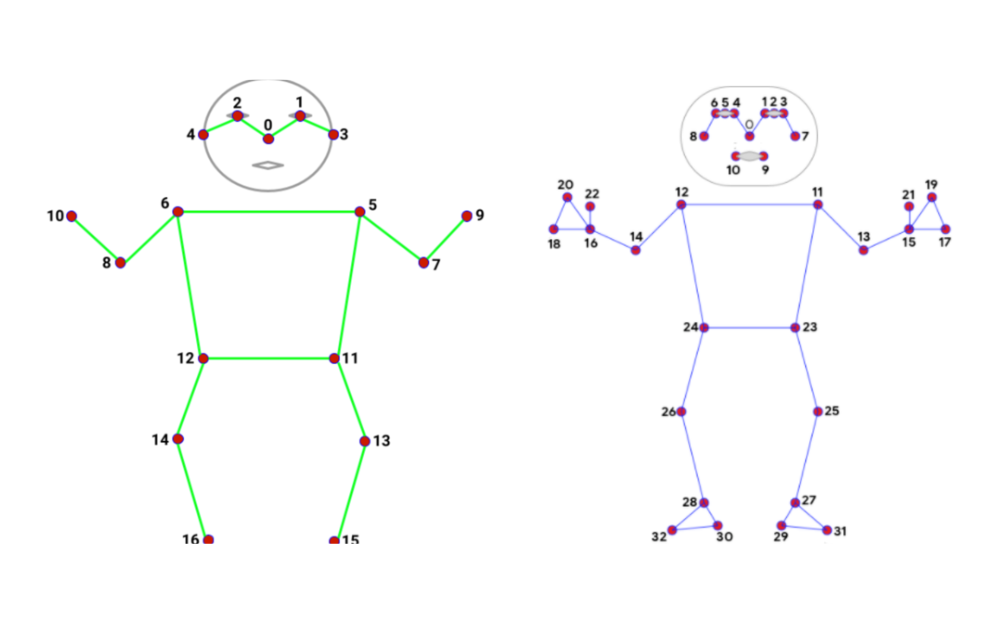
\includegraphics[width=\linewidth]{img/hpe_keypoints.png}
    \caption{Comparativa de les topologies anatòmiques estandarditzades en \textit{Human Pose Estimation} (\textit{HPE}). A l'esquerra, l'esquelet \textit{COCO} (17 punts); a la dreta, l'esquelet \textit{BlazePose} (33 punts).}
    \label{fig:keypoint_mapping}
\end{figure}

En rebre el JSON amb les coordenades normalitzades de Sapiens, s'executa una funció de mapeig que s'encarrega d'identificar els índexs de COCO i reescriure'ls en les posicions corresponents de la topologia de MediaPipe, generant un nou esquelet normalitzat. Aquest pas d'estandardització ha estat la clau per aprofitar la superioritat biomecànica del model \textit{Sapiens-2B} sense haver de reescriure tota la lògica d'avaluació geomètrica inicialment programada, garantint un esquelet de 33 punts de control (peus inclosos) aïllat del model de detecció subjacent.

\subsection{Pipeline d'Extracció i Suavitzat Temporal}
Un cop seleccionat el model, s'ha implementat el mòdul de processament de senyal per mitigar el soroll de l'estimació. Un element de debat tecnològic en aquesta fase ha estat l'ús del filtre de \textit{Savitzky-Golay}. 

Aquest algorisme es basa en l'ajust local d'un polinomi sobre una finestra de dades de mida $n = 2m+1$. Seguint el formalisme del model d'optimització de pesos per a aquest filtre, l'objectiu és determinar els coeficients $c_j$ que minimitzin la variància de l'error en el senyal suavitzat. L'error quadràtic mitjà ($E$) a minimitzar dins de la finestra es defineix com:

\begin{equation}
    E = \sum_{i=-m}^{m} w_i \left( p(i) - x_i \right)^2
\end{equation}

On $p(i)$ és el polinomi d'ajust i $x_i$ les coordenades originals. Aquesta minimització és equivalent a optimitzar la propagació de la variància $\sigma^2_{\Delta e}$ a través dels coeficients del filtre, assegurant que el suavitzat no elimini la informació pertinent del moviment.

A causa dels primers resultats obtinguts, es va valorar la possibilitat de suprimir-lo, ja que en moviments d'alta freqüència o auto-oclusions severes, la regressió intentava suavitzar trajectòries incoherents, provocant deformacions en l'esquelet virtual.

\begin{figure}[H]
    \centering
    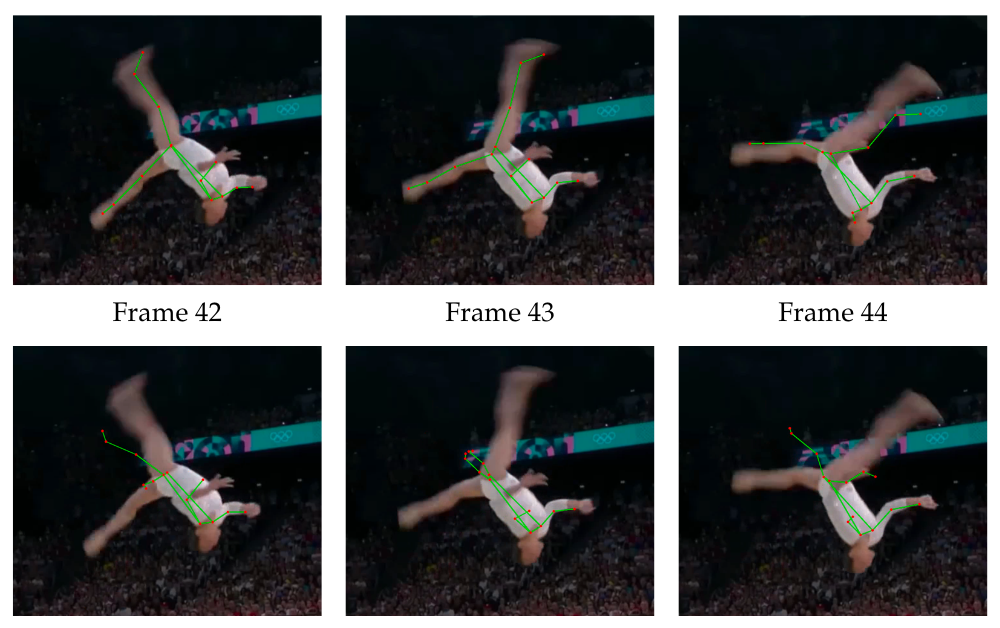
\includegraphics[width=\linewidth]{img/compare_smooth_bad.png}
    \caption{Exemple d'efecte no desitjat (\textit{oversmoothing}) en l'extracció de coordenades durant un gir de perfil (figura inferior). El filtre de Savitzky-Golay difumina l'intercanvi de cames provocant una pèrdua de la morfologia real.}
    \label{fig:compare_bad}
\end{figure}

No obstant això, aquesta decisió es va revertir en comprovar la seva importància crítica per a l'estabilitat global del sistema. Durant les extraccions massives per al \textit{dataset} d'entrenament de la \textit{RNN} i els tests de l'\textit{E-Score}, s'ha demostrat que l'aplicació del filtre és fonamental per retenir \textit{frames} on la confiança de la xarxa descendeix fins no mostrar cap esquelet en el \textit{frame} (\textit{frame dropping}). En acrobàcies d'extensió fluida, el filtre assoleix un alineament biomecànic quasi perfecte.

\begin{figure}[H]
    \centering
    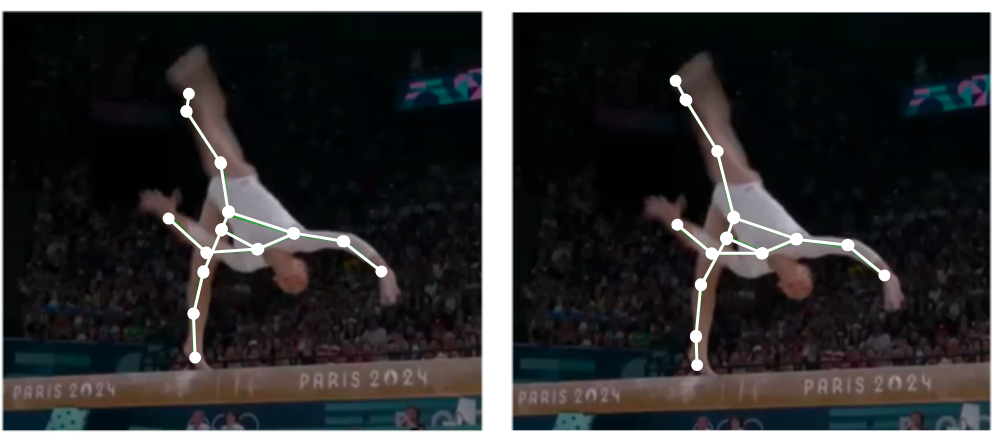
\includegraphics[width=\linewidth]{img/compare_smooth_good.png}
    \caption{Exemple de comportament òptim del filtre en moviments parabòlics. L'esquelet (a baix) presenta una coherència biomecànica superior al resultat en cru (\textit{raw}) del fragment de vídeo processat (a dalt).}
    \label{fig:compare_good}
\end{figure}

Aquesta dualitat de resultats ha permès concloure que els beneficis en l'estabilitat temporal superen els riscos puntuals de deformació. Per tant, s'ha optat per procedir amb l'algorisme per garantire un senyal espacial continu per al motor de regles.

\subsection{Creació del Dataset i Data Augmentation}
L'entrenament d'un classificador basat en xarxes recurrents exigeix un volum de dades representatiu i equilibrat. Per a la construcció del \textit{dataset} d'aquest projecte, s'han seleccionat majoritàriament vídeos procedents del canal oficial de \textit{USA Gymnastics}\cite{usa_gymnastics_yt}, identificant i retallant fragments de rutines de barra d'equilibris (\textit{Balance Beam}). L'objectiu ha estat aïllar la fase aèria de les quatre categories acrobàtiques definides, el comportament morfològic de les quals es recopila visualment a la Figura \ref{fig:exercises}. A partir d'aquestes rutines, s'ha obtingut una mostra inicial de 72 seqüències homogènies.

\begin{figure}[H]
    \centering
    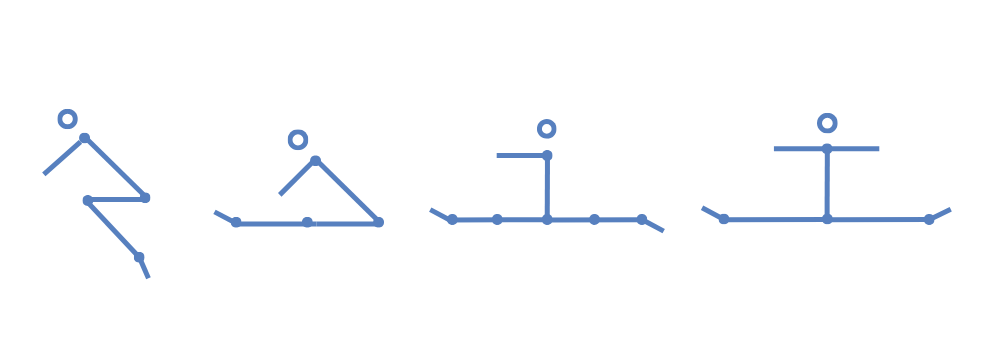
\includegraphics[width=\linewidth]{img/exercises.png}
    \caption{Representació de les quatre categories de salts analitzades. D'esquerra a dreta: Tuck (salt agrupat); Pike (salt carpat); Split (salt amb obertura lateral); Straddle (salt amb obertura frontal).}
    \label{fig:exercises}
\end{figure}

Atès el volum limitat d'aquest conjunt original, s'ha implementat un mòdul de \textit{Data Augmentation} per augmentar artificialment la mida del \textit{dataset} i millorar la capacitat de generalització del model. La tècnica principal ha consistit en la generació de dades sintètiques mitjançant un efecte de mirall (\textit{mirroring}). A diferència d'altres sistemes que inverteixen el vídeo original, aquest algorisme aplica una transformació lineal directament sobre l'eix X de les coordenades JSON ja exportades, invertint la seva posició respecte al centre del tors.

Aquesta operació ensenya a la xarxa a reconèixer la simetria biomecànica de l'exercici independentment de l'orientació del salt, i ha permès duplicar exactament el volum de dades per a cada categoria, aconseguint un \textit{dataset} final constituït per un total de 144 mostres estructurades (vegeu la Taula \ref{tab:dataset_stats}).

\begin{table}[H]
\centering
\caption{Distribució del dataset d'entrenament per categoria}
\label{tab:dataset_stats}
\renewcommand{\arraystretch}{1.3}
\begin{tabular}{lcc}
\hline
\textbf{Categoria} & \textbf{Mostres Originals} & \textbf{Total Dades} \\ \hline
\textit{\textbf{Pike}}     & 18 & 36 \\
\textit{\textbf{Split}}    & 20 & 40 \\
\textit{\textbf{Straddle}} & 17 & 34 \\
\textit{\textbf{Tuck}}     & 17 & 34 \\ \hline
\textbf{TOTAL}    & \textbf{72} & \textbf{144} \\ \hline
\end{tabular}
\end{table}

Aquestes seqüències temporals de 30 \textit{frames} s'utilitzen per alimentar una xarxa neuronal recurrent (\textit{RNN}) basada en capes \textit{Long Short-Term Memory} (\textit{LSTM}), l'arquitectura de la qual es detalla a la Figura \ref{fig:lstm}. Aquest tipus de capa és ideal per processar sèries temporals cinemàtiques, ja que resol el problema del \textit{Vanishing Gradient} (el gradients disminueixen fins no actualitzar els pesos de la xarxa) mitjançant un mecanisme de portes rutes. 

Específicament, per a cada interval de temps $t$, el vector de coordenades d'entrada $x_t$ i l'estat ocult anterior $h_{t-1}$ són processats de forma seqüencial. La porta d'oblit (\textit{forget gate}, $F_t$) determina quina informació històrica es descarta, mentre que la porta d'entrada (\textit{input gate}, $I_t$) i l'estat de cel·la candidat ($\tilde{C}_t$) regulen la incorporació dels nous patrons cinemàtics per actualitzar la memòria de la cel·la ($C_t$). Finalment, la porta de sortida (\textit{output gate}, $O_t$) modula el nou estat ocult $h_t$, encarregat d'enviar la informació cap a la capa de classificació final per discernir l'acrobàcia executada.

\begin{figure}[H]
    \centering
    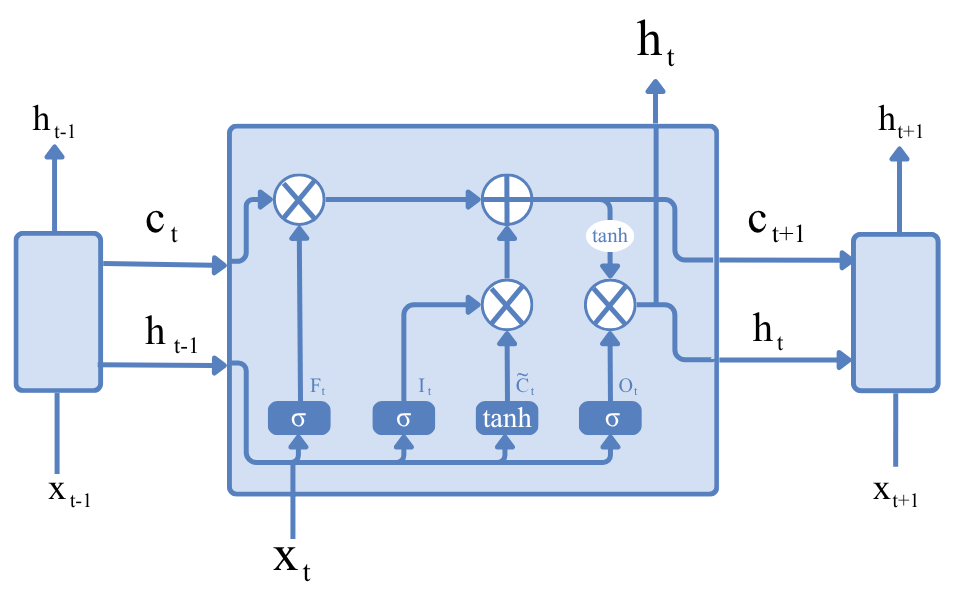
\includegraphics[width=\linewidth]{img/lstm.png}
    \caption{Arquitectura d'un bloc recurrent LSTM, on es detalla el flux temporal controlat per les portes d'oblit ($F_t$), entrada ($I_t$), sortida ($O_t$) i la cel·la de memòria candidat ($\tilde{C}_t$).}
    \label{fig:lstm}
\end{figure}

\subsection{Motor de Lògica d'Avaluació i Pelvis Virtual}
Una vegada la xarxa \textit{LSTM} ha classificat l'acrobàcia, el sistema transfereix el control al mòdul \textit{AcrobaticEvaluator}. Aquest component actua com un motor determinista que tradueix les normatives del Codi de Puntuació de la \textit{FIG} \cite{fig_rules} en regles geomètriques computables. La responsabilitat d'aquest motor es troba en identificar el \textit{peak frame} (\textit{frame} de màxima amplitud) i aplicar-hi els llindars de penalització definits al mòdul \texttt{rules.py}.

Per garantir una avaluació robusta davant la distorsió de la perspectiva monocular, s'ha dissenyat la Pelvis Virtual. Es tracta d'un punt de control sintètic, que anomenarem punt imaginari ($P_i$), calculat com el punt mig geomètric entre els \textit{keypoints} dels malucs esquerre ($P_L$) i dret ($P_R$), corresponents als índexs 23 i 24 de l'arquitectura d'extracció:

\begin{equation}
    P_i = \left( \frac{x_L + x_R}{2}, \frac{y_L + y_R}{2} \right)
\end{equation}

Aquest $P_i$ permet establir un origen de coordenades invariant a la rotació de la gimnasta. Per calcular l'amplitud d'obertura o flexió, el sistema construeix dos vectors, $\vec{u}$ i $\vec{v}$, que connecten el punt virtual amb les articulacions adjacents (per exemple, els genolls $K_L$ i $K_R$ en el cas d'un \textit{split}):

\begin{equation}
    \vec{u} = K_L - P_i, \quad \vec{v} = K_R - P_i
\end{equation}

L'angle real d'obertura $\theta$ s'obté mitjançant l'aplicació de la fórmula del producte escalar per extreure l'angle entre ambdós vectors:

\begin{equation}
    \theta = \arccos\left(\frac{\vec{u} \cdot \vec{v}}{|\vec{u}| |\vec{v}|}\right) \cdot \frac{180}{\pi}
\end{equation}

Atès que l'execució biomecànica real presenta variabilitats naturals i que els valors ideals (com els 180º en un \textit{split} o els 45º en un \textit{tuck}) són fites de perfecció absoluta, s'han adaptat els llindars de penalització. Aquesta calibració permet que el sistema no sigui excessivament punitiu, mantenint la fidelitat a la documentació original però ajustant-se a la realitat del moviment humà. A la Taula \ref{tab:thresholds} es detallen els llindars angulars implementats per a cada deducció.

\begin{table}[H]
\centering
\caption{Llindars angulars i deduccions aplicades (\textit{E-Score})}
\label{tab:thresholds}
\renewcommand{\arraystretch}{1.5}
\begin{tabular}{l p{1.25cm} ccc}
\hline
\textbf{Acrobàcia} & \textbf{Criteri} & \textbf{Minor} & \textbf{Medium} & \textbf{Severe} \\ 
 & & (-0.1) & (-0.3) & (-0.5) \\ \hline
\textit{\textbf{Tuck}} & \textit{Hip} \newline \textit{Knee} & $< 65^\circ$ & $< 90^\circ$ & $< 100^\circ$ \\ \hline
\textit{\textbf{Pike}} & \textit{Hip} & $< 65^\circ$ & $< 90^\circ$ & $< 100^\circ$ \\
 & \textit{Knee} & $> 170^\circ$ & $> 160^\circ$ & $> 145^\circ$ \\ \hline
\textit{\textbf{Split}} & \textit{Opening} & $> 170^\circ$ & $> 160^\circ$ & $> 135^\circ$ \\
 & \textit{Knee} & $> 170^\circ$ & $> 160^\circ$ & $> 145^\circ$ \\ \hline
\textit{\textbf{Straddle}} & \textit{Opening} & $> 170^\circ$ & $> 160^\circ$ & $> 135^\circ$ \\
 & \textit{Knee} & $> 170^\circ$ & $> 160^\circ$ & $> 145^\circ$ \\ \hline
\end{tabular}
\end{table}

Aquests llindars es vinculen directament al sistema de visualització mitjançant un mapeig de colors (\textit{Color Map}): les infraccions \textit{Minor} es representen en verd, les \textit{Medium} en taronja i les \textit{Severe} en vermell. El sistema calcula la desviació del \textit{frame} pic respecte a la base de 10.0 punts, oferint un desglossament objectiu que el jutge pot validar mitjançant la futura interfície de \textit{PyQt6}.

\subsection{Avaluació Contínua i Mapeig Espacial}
Per tal de transcendir l'anàlisi de clips aïllats i permetre el processament de rutines completes, s'ha implementat un algorisme de finestra lliscant (\textit{sliding window}). Aquest sistema fragmenta el flux continu de vídeo en blocs temporals de $N=30$ \textit{frames} amb un desplaçament constant. Cada bloc s'envia a la xarxa \textit{LSTM}, que retorna una probabilitat de pertinença a les classes acrobàtiques.

Un repte detectat en aquesta fase d'avaluació contínua és la detecció de falsos positius en segments de transició, especialment durant els aterratges (\textit{landings}). Atès que el \textit{dataset} d'entrenament inclou la fase final del salt per captar la biomecànica completa, el model pot classificar erròniament el contacte amb la barra com a part de l'acrobàcia. Aquesta limitació es podria mitigar en línies futures amb la creació d'una nova classe a classificar per la xarxa neuronal, com ara \textit{"Transition"}, dissenyada específicament per captar els instants estructurals on la gimnasta inicia o finalitza el contacte amb l'aparell. No obstant això, cal subratllar que el sistema s'ha concebut com una eina d'assistència al judici: el jutge humà manté el criteri final i pot descartar aquelles avaluacions automàtiques que corresponguin a \textit{frames} no rellevants biomecànicament.

D'altra banda, per visualitzar les penalitzacions de forma clara, s'ha resolt el repte del mapeig espacial de coordenades. Les dades emmagatzemades al JSON són valors normalitzats relatius al centre del tors (en un rang aproximat de $[-1, 1]$), un format optimitzat per a l'aprenentatge del model de classificació profunda però no apte per a la representació gràfica directa. Per resoldre-ho, s'ha definit un llenç de representació normalitzat i s'ha implementat una funció de desnormalització lineal:

\begin{equation}
    X_{pixel} = (x_{norm} \cdot S) + O_x, \quad Y_{pixel} = (y_{norm} \cdot S) + O_y
\end{equation}

On $S$ és un factor d'escala constant per amplificar la magnitud de l'esquelet i $(O_x, O_y)$ representen l'\textit{offset} necessari per centrar la figura en el pla bidimensional. Aquesta transformació permet reconstruir l'esquelet virtual amb una proporció biomecànica perfecta, facilitant la il·luminació dinàmica dels \textit{joints} infractors (verd, taronja i vermell) segons la gravetat de la deducció calculada pel motor.

\subsection{Prototipatge de la Interfície Gràfica (GUI)}
Com a avançament estratègic de la Fase 4 del cronograma, dedicada al poliment i integració a l'aplicació d'escriptori per als jutges, s'ha iniciat el disseny de la interfície mitjançant el \textit{framework} \textit{PyQt6}. Cal subratllar que el mòdul es troba actualment en una fase de prototipatge visual no funcional, servint com a guia conceptual per validar la distribució d'elements abans de la seva implementació lògica final, així com per consolidar la familiarització pràctica amb les eines de programació seleccionades.

L'arquitectura prevista per a la interfície es fonamenta en un sistema de doble visualització (\textit{Dual Viewport}):

\begin{itemize}
    \item \textbf{Panell de Referència i Control:} Està destinat a la visualització del flux de vídeo principal. Es preveu que l'usuari pugui alternar dinàmicament entre tres modalitats crítiques: el metratge original de la competició, l'output directe del model \textit{Sapiens} (esquelet en cru renderitzat sobre el fitxer .avi) o la representació avançada que integra el codi de colors segons la gravetat de cada angle biomecànic obtingut de les metadades JSON.

    \item \textbf{Panell d'Anàlisi Biomecànic:} En aquest espai es renderitzarà l'esquelet virtual sobre el llenç linealitzat. Aquesta vista aïllada permet identificar les infraccions posturals de forma neta, utilitzant la il·luminació dinàmica de les articulacions per ressaltar les deduccions detectades pel motor de regles.
\end{itemize}

Així mateix, s'ha dissenyat un prototip d'aplicació d'escriptori (vegeu la Figura \ref{fig:gui_mockup}) que, en versions futures, comunicarà els resultats del motor de lògica en temps real. L'aplicació prioritza de forma paral·lela la visualització del \textit{frame} actual del vídeo i la llegibilitat en forma de \textit{log} de registre asíncron per a les deduccions aplicades en aquell instant concret del salt.

Aquest enfocament reafirma la visió del projecte com una eina d'assistència: la interfície es concep perquè la intel·ligència artificial actuï com un observador perifèric que proposa correccions, deixant sempre la potestat final de confirmar o descartar les penalitzacions al criteri expert del jutge humà.

\begin{figure}[H]
    \centering
    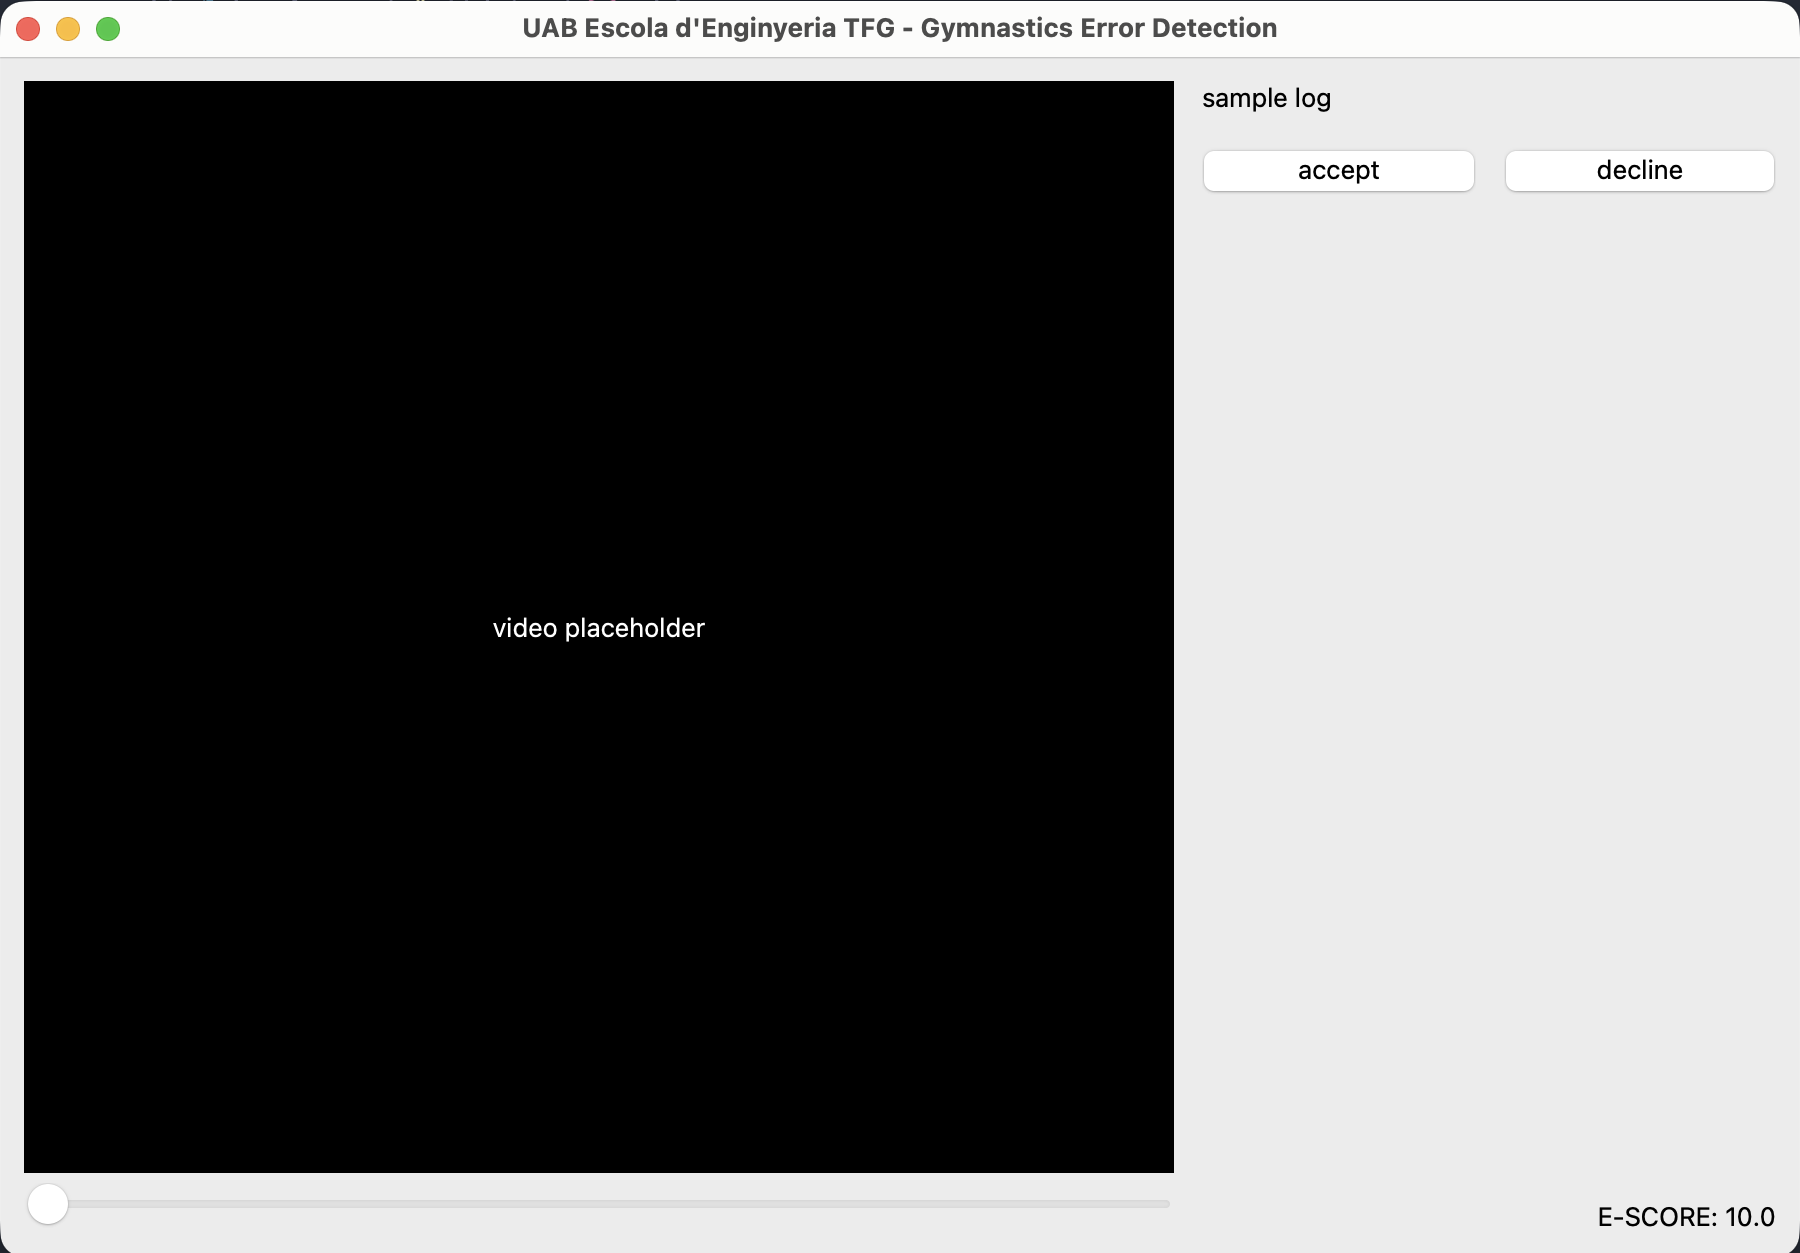
\includegraphics[width=0.9\linewidth]{img/mockup.png}
    \caption{Disseny conceptual (\textit{mockup}) de la interfície gràfica. Aquesta versió preliminar serveix per definir l'arquitectura visual i la disposició dels registres d'avaluació en forma de log de cara a la integració final a la Fase 4.}
    \label{fig:gui_mockup}
\end{figure}

\section{Resultats i Discussió}
Aquesta secció presenta els resultats experimentals obtinguts en la validació del sistema, dividits en l'avaluació quantitativa del model de classificació recurrent i l'anàlisi de comportament del motor de puntuació biomecànica sobre rutines reals.

\subsection{Rendiment del Classificador Recurrent (LSTM)}
Per avaluar la capacitat de la xarxa \textit{LSTM} per discriminar entre les quatre categories acrobàtiques (\textit{Pike, Split, Straddle, Tuck}), es va separar el \textit{dataset} final (144 mostres) en un 80\% d'entrenament i un 20\% de test independent. El rendiment del model s'ha mesurat mitjançant les mètriques clàssiques de Visió per Computador: Precisió (\textit{Precision}), Sensibilitat (\textit{Recall}) i la puntuació \textit{F1-Score}.

A la Taula \ref{tab:metrics_lstm} es detalla el comportament del classificador. Els resultats demostren una alta fiabilitat general, especialment en les classes \textit{Tuck} i \textit{Pike}, on la morfologia de l'esquelet és altament divergent de la resta.

\begin{table}[H]
\centering
\caption{Mètriques de rendiment de l'arquitectura LSTM per classe}
\label{tab:metrics_lstm}
\renewcommand{\arraystretch}{1.2}
\begin{tabular}{lccc}
\hline
\textbf{Categoria} & \textbf{Precision} & \textbf{Recall} & \textbf{F1-Score} \\ \hline
\textit{\textbf{Pike}}     & 100.0\% & 100.0\% & 100.0\% \\
\textit{\textbf{Split}}    & 75.0\%  & 33.0\%  & 46.0\%  \\
\textit{\textbf{Straddle}} & 33.0\%  & 75.0\%  & 46.0\%  \\
\textit{\textbf{Tuck}}     & 100.0\% & 100.0\% & 100.0\% \\ \hline
\textbf{Mitjana Ponderada} & \textbf{83.0\%}  & \textbf{76.0\%}  & \textbf{76.0\%}  \\ \hline
\end{tabular}
\end{table}

Per analitzar on es produeixen les confusions del model, s'ha generat la matriu de confusió (vegeu la Figura \ref{fig:confusion_matrix}). Els indicadors numèrics corroboren de manera empírica la hipòtesi plantejada a la metodologia: el principal repte de la xarxa recau en la degradació mútua entre les classes \textit{Split} i \textit{Straddle} (amb un \textit{F1-Score} simètric del 46.0\%). Aquest comportament és biomecànicament lògic, ja que ambdues acrobàcies impliquen una obertura de cames nominalment propera als 180º i el model basat en vídeo monocular pateix per distingir la direcció de l'obertura a causa de la pèrdua de profunditat tridimensional inherent a la perspectiva lateral. 

Com a millora futura, la incorporació d'una característica addicional d'orientació (\textit{orientation}), que complementi les mètriques actuals de posició, velocitat, acceleració i angles dins del vector d'entrada de la \textit{LSTM}, solucionaria potencialment aquest problema, aportant al classificador el context espacial necessari per discernir amb precisió el pla d'execució del salt.

\begin{figure}[H]
    \centering
    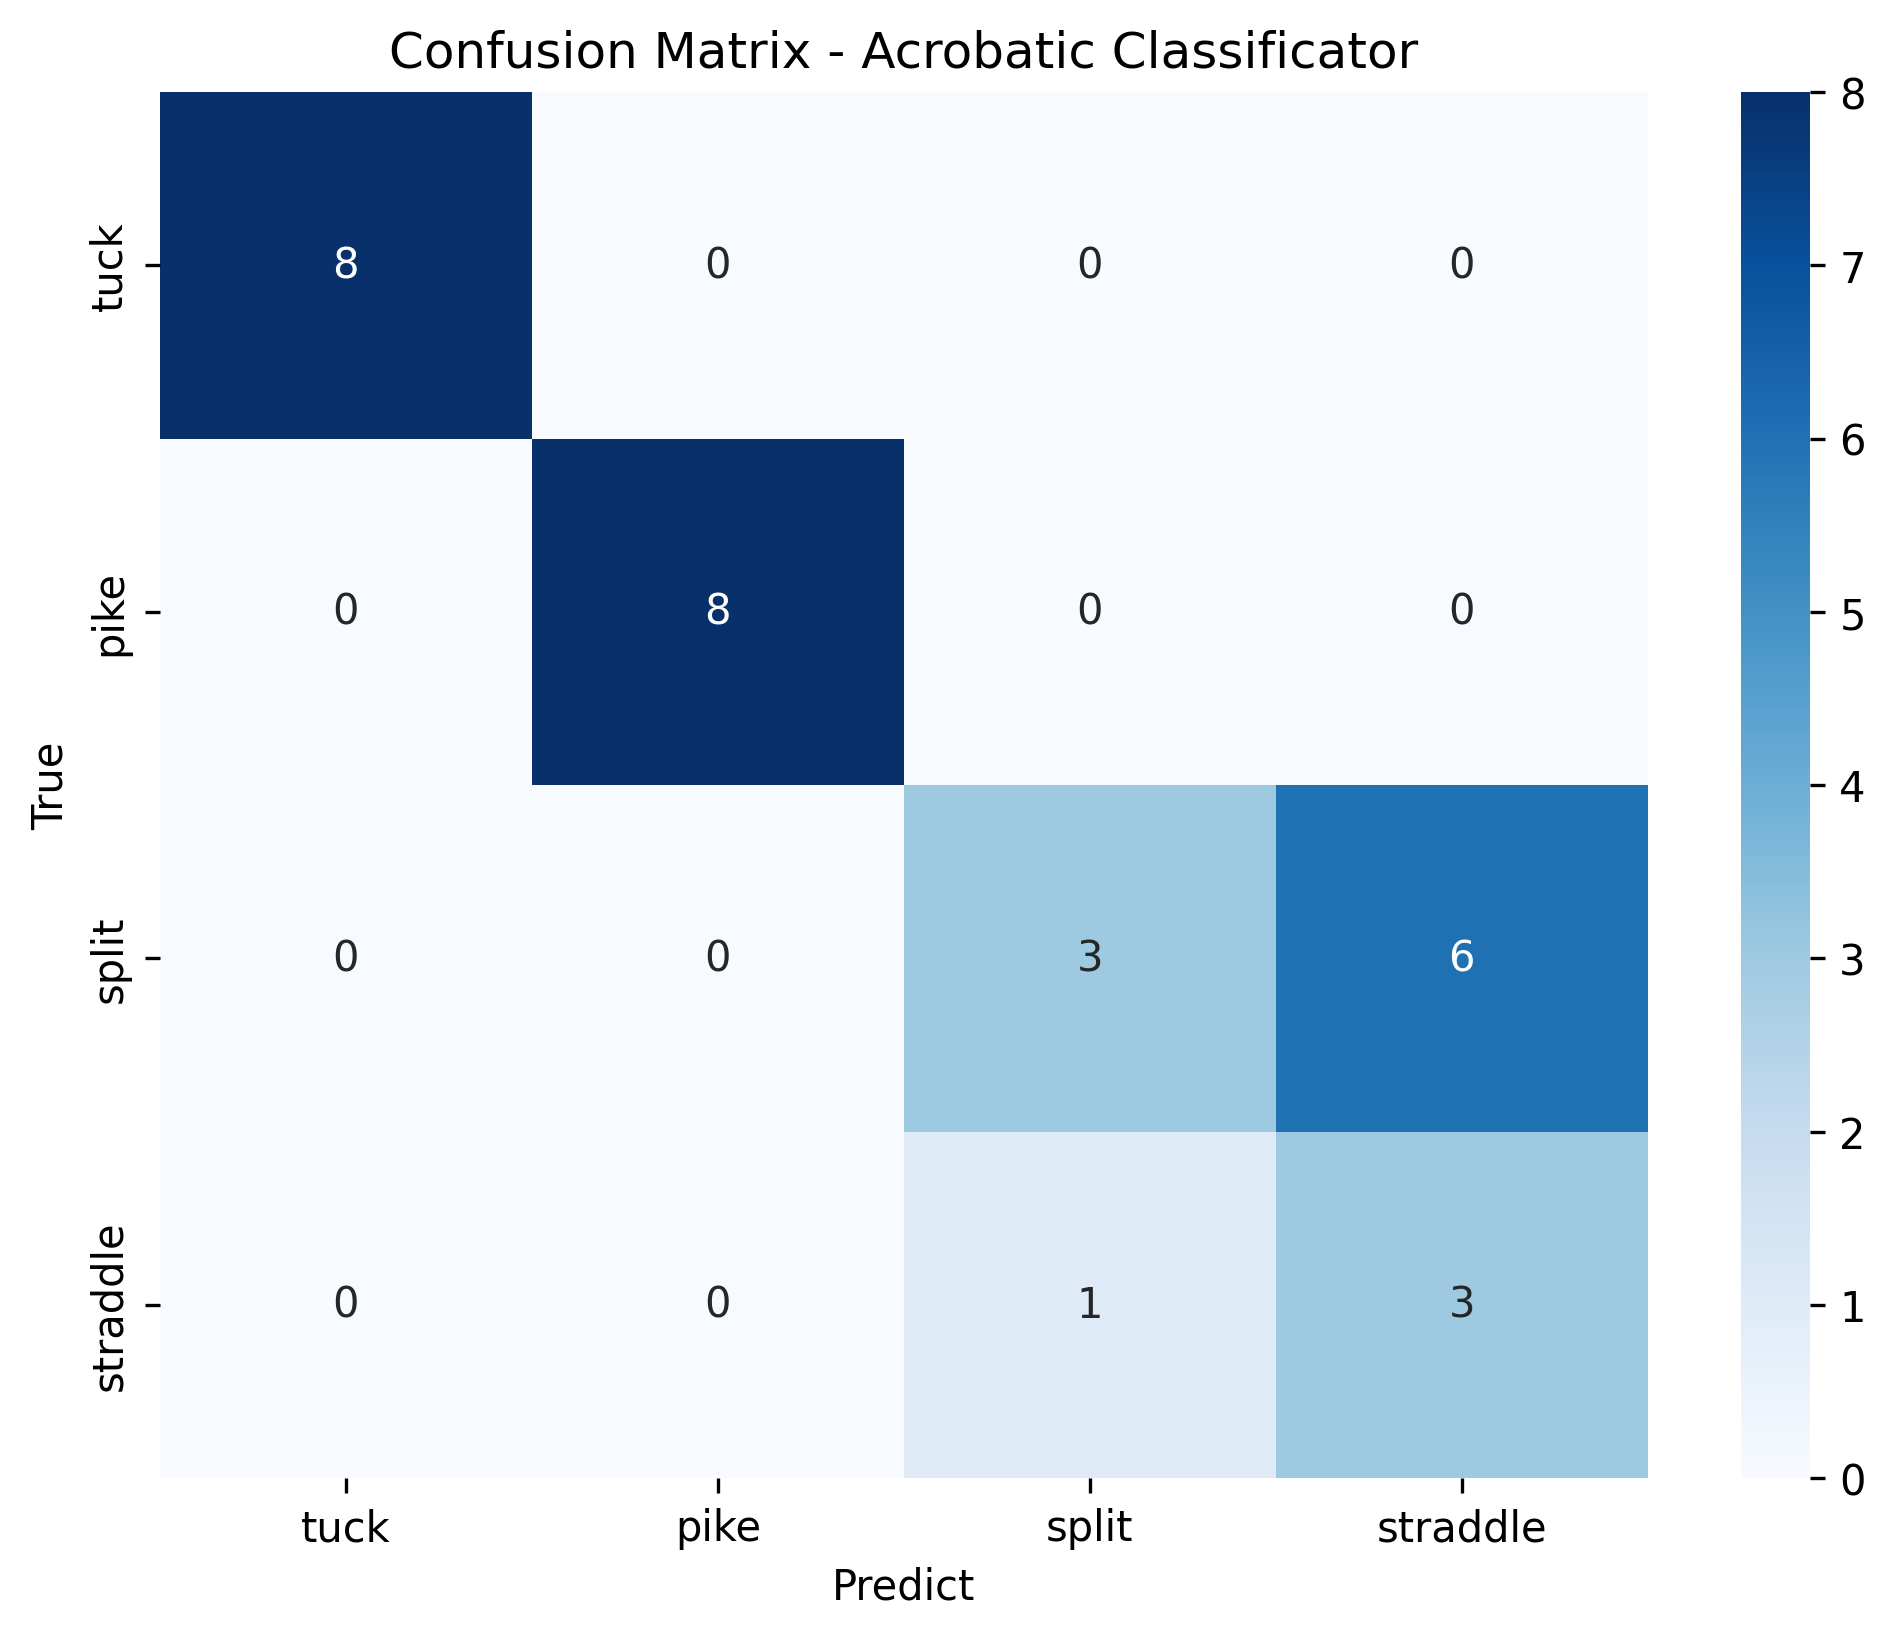
\includegraphics[width=0.8\linewidth]{img/model_confusion_matrix.png}
    \caption{Matriu de confusió del model LSTM sobre el conjunt de test. Es manifesta la lleugera ambigüitat lineal entre les classes d'obertura aèria.}
    \label{fig:confusion_matrix}
\end{figure}

\subsection{Validació de l'E-Score i Anàlisi de Casos Gràfics}
Una vegada validada la classificació, es va testejar la precisió del motor de lògica determinista sobre seqüències reals d'alta velocitat per avaluar l'aïllament de l'esquelet i el comportament del sistema de deduccions basat en el Codi de Puntuació de la \textit{FIG}. L'experimentació ha permès identificar dues tipologies de comportament del sistema:

\textbf{1) Funcionament Òptim i Captura de \textit{Peak Frame}:} La Figura \ref{fig:result_good} exemplifica el comportament ideal del \textit{pipeline}. El model \textit{LSTM} classifica correctament l'acrobàcia i el mòdul d'avaluació localitza amb precisió el \textit{frame} de màxima amplitud. El panell d'anàlisi biomecànic renderitza l'esquelet net on s'imprimeixen el tipus de salt i la seva confiança. A més, gràcies a l'algorisme de dibuix per capes amb prioritat de gravetat, s'il·luminen correctament en color vermell aquelles línies de control que superen els llindars crítics (penalització \textit{Severe}), garantint una traçabilitat visual immediata per al jutge.

\begin{figure}[H]
    \centering
    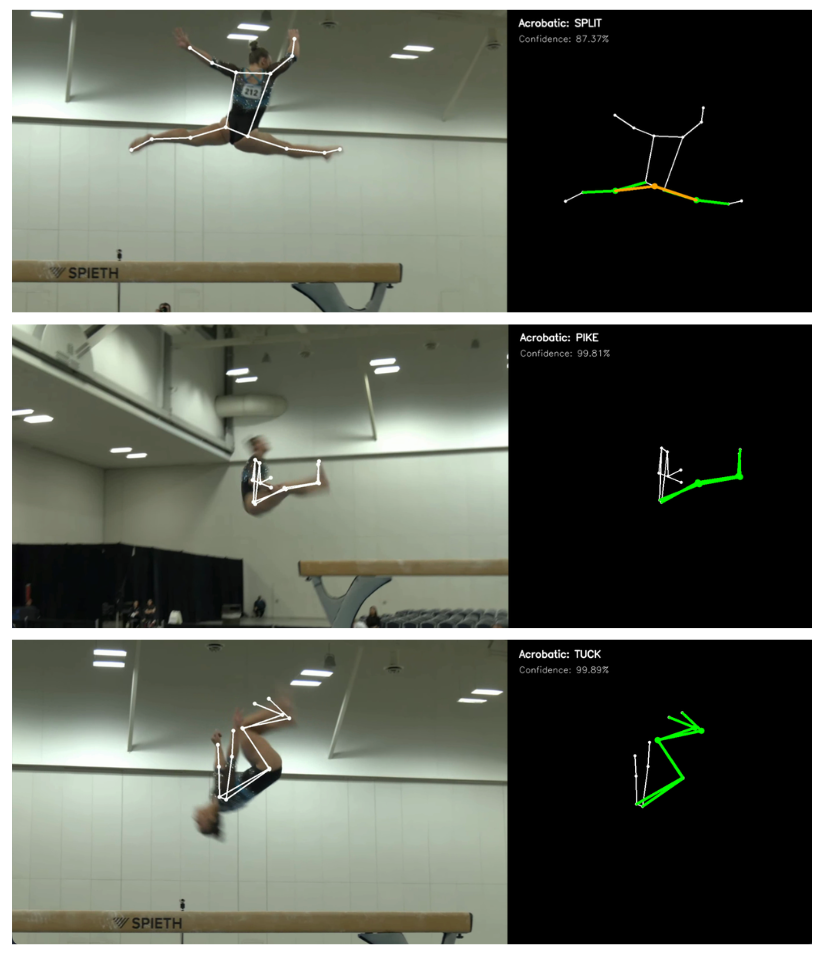
\includegraphics[width=\linewidth]{img/result_good.png}
    \caption{Visualització d'un cas d'èxit. L'esquelet es renderitza sobre el llenç reflectint de forma correcta les obertures angulars i superposant amb èxit la prioritat del color de penalització més greu.}
    \label{fig:result_good}
\end{figure}

\textbf{2) Propagació de l'Error per Fals Positiu de Transició:} Per contra, la Figura \ref{fig:result_bad} il·lustra un cas de fallada estructural causat per les limitacions temporals discutides. En aquest escenari, la xarxa \textit{LSTM} genera un fals positiu en classificar un fragment de transició (l'aterratge de la gimnasta) com una classe acrobàtica activa. 

És important matisar que el motor geomètric de l'\textit{AcrobaticEvaluator} actua de forma analíticament correcta: calcula els vectors sobre l'esquelet rebut i, en detectar angles completament tancats o deformats per l'impacte amb l'aparell, aplica de manera coherent una deducció de caràcter \textit{Severe} (-0.5). Per tant, la fallada no recau en la lògica matemática de les regles (que executa correctament el codi de colors vermell), sinó en una classificació errònia d'origen temporal que enganya el motor de regles.

\begin{figure}[H]
    \centering
    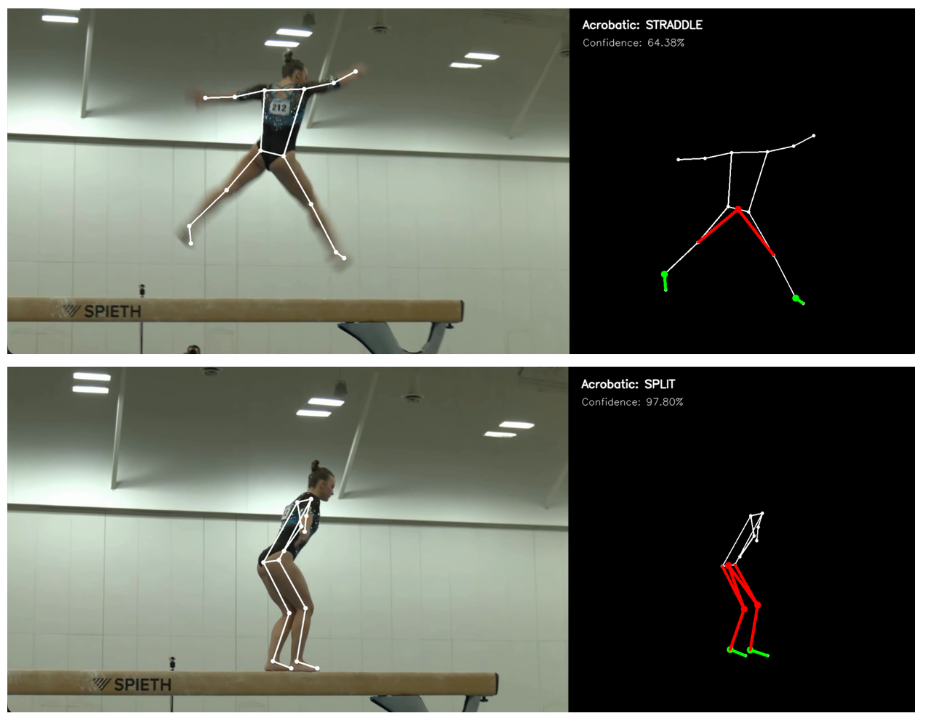
\includegraphics[width=\linewidth]{img/result_bad.png}
    \caption{Visualització d'un cas crític de fals positiu. S'observa l'aplicació d'una penalització severa provocada per una activació errònia de la LSTM durant la fase de recepció o contacte amb la barra.}
    \label{fig:result_bad}
\end{figure}

\subsection{Anàlisi de l'Avaluació Contínua i Eficiència Temporal}
El comportament de la finestra lliscant (\textit{sliding window}) ha permès extreure de manera contínua múltiples acrobàcies en un sol flux de vídeo sense necessitat de segmentació manual prèvia. L'aparició d'anomalies com la mostrada a la Figura \ref{fig:result_bad} reforça la decisió de dissenyar el sistema sota el paradigma d'eina d'assistència: en ser el \textit{log} de registres un sistema interactiu, el jutge humà pot identificar instantàniament si una penalització prové d'un frame d'aterratge i invalidar-la prement la interfície, actuant com el filtre de control de qualitat definitiu.
Finalment, s'ha realitzat un estudio de la latència i la viabilitat computacional del \textit{pipeline}. En un entorn de proves equipat amb una GPU \textit{NVIDIA GeForce RTX 2080 Ti}, un maquinari de consum de generacions anteriors que actua com un banc de proves modest pel volum del model, el processament complet d'un fragment de rutina d'1 minut i 20 segons gravat a 30 fps (2.400 \textit{frames}) requereix aproximadament entre 3 i 4 hores d'inferència contínua. Això es tradueix en un cost proper als 5 o 6 segons per \textit{frame} per a l'extracció massiva amb \textit{Sapiens-2B}, el processament de senyal i l'avaluació de l'\textit{E-Score}.

Aquestes dades posen de manifest un dels grans compromisos en l'àmbit de la Visió per Computador: la priorització absoluta de la precisió i la robustesa biomecànica enfront de la velocitat de procés. \textit{Sapiens-2B} es un model fundacional a gran escala (2 mil milions de paràmetres) que exigeix una gran capacitat de còmput, una envergadura que justifica aquest \textit{bottleneck} temporal, però que a canvi ofereix l'alta taxa d'encert davant d'oclusions severes descrita a la Taula \ref{tab:avaluacio-gym}.

D'aquesta manera, l'execució \textit{offline} esdevé una solució molt econòmica per a l'esport base. Permet als clubs de tecnificació prescindir de la infraestructura multimilionària de \textit{Fujitsu} i analitzar els vídeos de les sessions postcompetició o dels entrenaments de manera totalment assequible. 

Com a línies clau de treball futur per al projecte, es planteja l'optimització d'aquests temps de procés per dues vies: d'una banda, la migració del sistema cap a arquitectures de GPU actuals de gamma alta (com ara les sèries \textit{NVIDIA RTX 4090} o similars), les quals reduirien notablement el temps d'espera gràcies a la seva potència de còmput moderna. D'altra banda, es proposa l'exploració de models d'extracció de poses alternatius que siguin més lleugers, avaluant si és possible reduir la latència general del lliurament de dades sense sacrificar excessivament la fidelitat anatòmica de la gimnasta.

\section{Conclusions Provisionals}
A partir del desenvolupament i les proves de validació realitzades fins a la data, s'ha demostrat la viabilitat tècnica del sistema. Les principals conclusions es resumeixen en els següents punts:

\begin{itemize}
    \setlength{\itemsep}{0.5em} % Dona una mica més d'espai entre punts per evitar que quedi "enganxat"
    
    \item La combinació del model fundacional \textit{Sapiens-2B} amb la xarxa recurrent \textit{LSTM} s'ha consolidat com una arquitectura robusta per a l'anàlisi cinemàtica. Tot i l'ambigüitat inherent provocada per la pèrdua de profunditat de la visió monocular en els salts d'obertura (amb un \textit{F1-Score} del 46.0\% en \textit{Split} i \textit{Straddle}), l'èxit absolut del 100\% en les classes \textit{Tuck} i \textit{Pike} en valida el rendiment global.

    \item El disseny de la Pelvis Virtual com a punt de control sintètic ha demostrat ser una solució geomètrica eficaç. L'ús de vectors i productes escalars permet traduir les normatives de la \textit{FIG} de manera totalment objectiva i invariant respecte a la perspectiva lineal o rotació de la gimnasta.

    \item L'estudi de latència del \textit{pipeline} (entre 3 i 4 hores per a un vídeo de 2.400 \textit{frames} en una GPU \textit{NVIDIA RTX 2080 Ti}) confirma el compromís clàssic entre precisió biomecànica i temps de còmput. No obstant això, l'execució en diferit (\textit{offline}) compleix l'objectiu fonamental de democratitzar aquest tipus d'anàlisi, oferint una alternativa assequible per a l'esport base davant els sistemes multimilionaris de l'elit mundial.

    \item Es reafirma el paradigma del programari com una eina d'assistència i suport al judici, on la intel·ligència artificial actua com un observador algorísmic d'alta precisió per proposar deduccions de l'\textit{E-Score}, delegant sempre la potestat de la decisió final al criteri expert del jutge humà.
\end{itemize}

Com a línia de treball immediata per a la finalització del projecte, un cop tancada amb èxit la validació dels models lògics i d'intel·ligència artificial, es procedirà al desenvolupament i programació de la interfície gràfica interactiva definitiva mitjançant el \textit{framework} \textit{PyQt6}.

\section*{Ús de la IA Generativa}
En compliment de la normativa d'avaluació del Treball Final de Grau de la UAB, es declara que en l'elaboració d'aquest Informe de Progrés II s'han utilitzat eines d'Intel·ligència Artificial generativa (model \textit{Gemini 3 Pro}). 

D'acord amb les directrius establertes, el seu ús s'ha limitat exclusivament a l'assistència en aspectes formals i tècnics. Concretament, l'eina s'ha emprat per a la revisió ortotipogràfica, la millora de la fluïdesa i claredat expositiva de la redacció en català, i com a suport tècnic per a la resolució de problemes de formatació i estructuració del codi en llenguatge \LaTeX.

Es certifica que no s'ha utilitzat cap model generatiu per a la creació dels continguts intel·lectuals sotmesos a avaluació. La definició del context, l'establiment dels objectius, el disseny del \textit{pipeline} metodològic i la planificació temporal del projecte han estat elaborats de manera íntegrament autònoma per l'autora.

\begin{thebibliography}{99}

\bibitem{paris_2024}
La Vanguardia, \textit{Una gimnasta rumana recibe la medalla de bronce once días después de la final de los JJOO}, Agost 2024. [En línia]. Disponible a: \url{https://www.lavanguardia.com/deportes/20240817/9874948/gimnasta-recibe-medalla-bronce-once-dias-final-jjoo.html}

\bibitem{olympics_scoring}
International Olympic Committee (IOC), \textit{Artistic gymnastics scoring system and judging rules: The D-score and E-score explained}. [En línia]. Disponible a: \url{https://olympics.com/en/news/artistic-gymnastics-scoring-system-judging-rules-e-d-score}

\bibitem{fujitsu_jss}
Fujitsu, \textit{Judging Support System Co-development with FIG}. [En línia]. Disponible a: \url{https://www.fujitsu.com/global/themes/data-driven/judging-support-system/}

\bibitem{yolov8}
Ultralytics, \textit{YOLOv8 Pose Task Documentation}. [En línia]. Disponible a: \url{https://docs.ultralytics.com/tasks/pose/#predict}

\bibitem{sapiens_2024}
T. Rawal \textit{et al.} (Meta), \textit{Sapiens: Foundation for Human Vision Models}, arXiv preprint arXiv:2408.12569, 2024. Disponible a: \url{https://arxiv.org/abs/2408.12569}

\bibitem{mediapipe}
Google Research, \textit{MediaPipe: A Framework for Building Perception Pipelines}. Disponible a: \url{https://arxiv.org/pdf/1906.08172}

\bibitem{blazepose_2020}
V. Bazarevsky \textit{et al.} (Google), \textit{BlazePose: On-device Real-time Body Pose tracking}, CVPR Workshop on Computer Vision for Augmented and Virtual Reality, 2020. Disponible a: \url{https://arxiv.org/abs/2006.10204}

\bibitem{fig_rules}
Fédération Internationale de Gymnastique (FIG), \textit{2025-2028 Code of Points (MAG \& WAG)}. [En línia]. Disponible a: \url{https://www.gymnastics.sport/site/rules/}

\bibitem{cvat}
CVAT - Open Data Annotation Platform. [En línia]. Disponible a: \url{https://www.cvat.ai/}

\bibitem{usa_gymnastics_yt}
USA Gymnastics, \textit{USA Gymnastics Official YouTube Channel - Balance Beam Search results}. [En línia]. Disponible a: \url{https://www.youtube.com/@usagymnastics/search?query=balance%20beam}

\bibitem{partimagenet_2024}
X. Li, Y. Liu, N. Dong, S. Qin, and X. Hu, \textit{PartImageNet++ Dataset: Scaling up Part-based Models for Robust Recognition}, en European Conference on Computer Vision (ECCV), 2024. Disponible a: \url{https://arxiv.org/abs/2407.10918}

\bibitem{zheng_hpe_survey}
C. Zheng, W. Wu, C. Chen, T. Yang, S. Zhu, J. Shen, N. Kehtarnavaz, and M. Shah, \textit{Deep Learning-Based Human Pose Estimation: A Survey}, ACM Computing Surveys, vol. 56, no. 1, 2023. Disponible a: \url{https://arxiv.org/pdf/2012.13392}

\bibitem{deeppose_2014}
A. Toshev and C. Szegedy, \textit{DeepPose: Human pose estimation via deep neural networks}, en Proceedings of the IEEE Conference on Computer Vision and Pattern Recognition (CVPR), pp. 1653-1660, 2014. Disponible a: \url{https://arxiv.org/abs/1312.4659}

\bibitem{hrnet}
Microsoft Research, \textit{Deep High-Resolution Representation Learning for Human Pose Estimation}. Disponible a: \url{https://arxiv.org/pdf/1902.09212}

\bibitem{alphapose}
Hao-Shu Fang, \textit{AlphaPose: Whole-Body Regional Multi-Person Pose Estimation and Tracking in Real-Time}. Disponible a: \url{https://arxiv.org/pdf/2211.03375}

\bibitem{vitpose}
ViTAE-Transformer, \textit{ViTPose: Simple Vision Transformer Baselines for Human Pose Estimation}. GitHub. [En línia]. Disponible a: \url{https://github.com/ViTAE-Transformer/ViTPose}

\bibitem{yang_pck_2013}
Y. Yang and D. Ramanan, \textit{Articulated Human Detection with Flexible Mixtures of Parts}, IEEE Transactions on Pattern Analysis and Machine Intelligence, vol. 35, no. 12, pp. 2878-2890, 2013. Disponible a: \url{https://www.cs.cmu.edu/~deva/papers/pose_pami.pdf}

\bibitem{coco_dataset_2014}
T.Y. Lin \textit{et al.}, \textit{Microsoft COCO: Common Objects in Context}, en European Conference on Computer Vision (ECCV), pp. 740-755, 2014. Disponible a: \url{https://arxiv.org/abs/1405.0312}

\bibitem{yolo_oks}
D. Maji, S. Nagori, M. Mathew, and D. Poddar, \textit{YOLO-Pose: Enhancing YOLO for Multi Person Pose Estimation Using Object Keypoint Similarity Loss}, en IEEE/CVF Conference on Computer Vision and Pattern Recognition Workshops (CVPRW), 2022. Disponible a: \url{https://arxiv.org/abs/2204.06806}

\bibitem{savgol}
Paul W. Oxby, \textit{An Optimal Weighting Function for the Savitzky-Golay Filter}. Disponible a: \url{https://arxiv.org/pdf/2111.11667}

\bibitem{finegym}
D. Shao \textit{et al.}, \textit{FineGym: A Hierarchical Video Dataset for Fine-grained Action Understanding}. Disponible a: \url{https://arxiv.org/pdf/2004.06704}

\bibitem{lstm_rnn_2021}
C. B. Vennerød, A. Kjærran, and E. S. Bugge, \textit{Long Short-term Memory RNN}, arXiv preprint arXiv:2105.06756, 2021. Disponible a: \url{https://arxiv.org/pdf/2105.06756}

\end{thebibliography}

\clearpage
\onecolumn
\appendix

\clearpage
\section{Diagrama d'Arquitectura Modular}
\label{apx:arquitectura}

\begin{figure}[H]
    \centering
    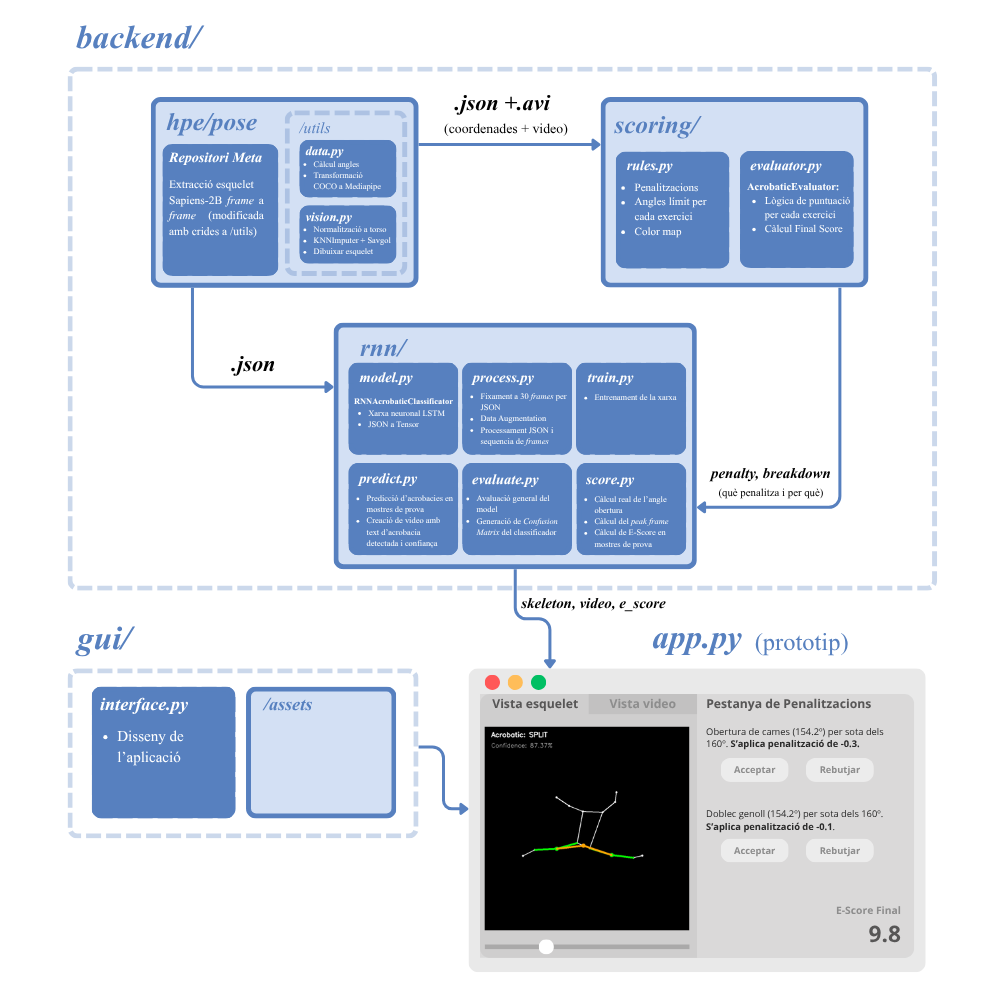
\includegraphics[width=0.9\linewidth]{img/diagrama.png}
    \caption{Diagrama complet d'arquitectura de programari i interacció de mòduls del sistema (HPE, RNN, Scoring i GUI). Elaboració pròpia mitjançant \textit{Canva}.}
    \label{fig:architecture_diagram}
\end{figure}

\clearpage
\section{Diagrama de Gantt}
\label{apx:gantt}

\begin{figure}[h]
    \centering
    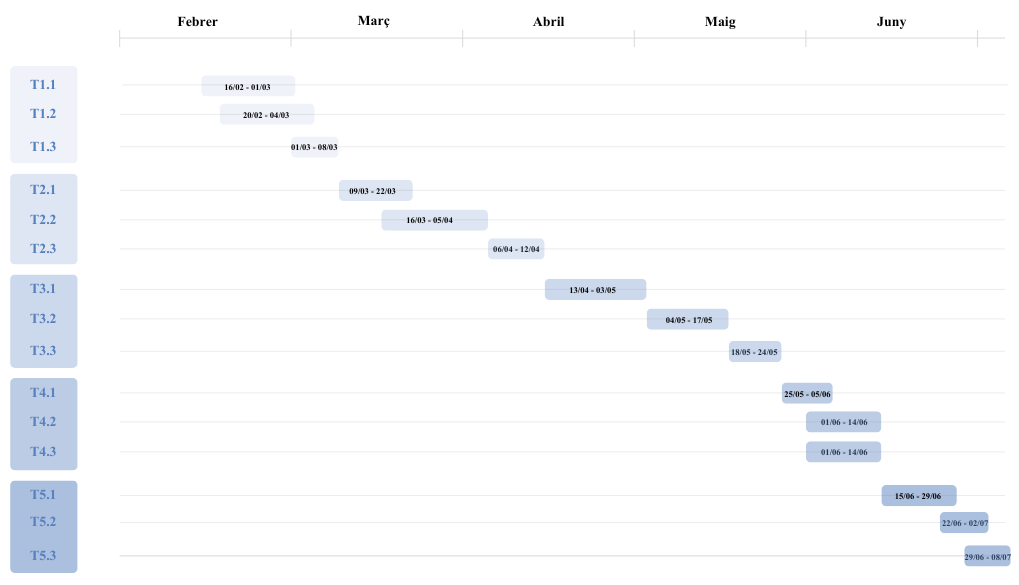
\includegraphics[width=\linewidth]{img/gantt.png}
    \caption{Cronograma del projecte (Diagrama de Gantt). Elaboració pròpia mitjançant \textit{Canva} a partir de la planificació feta a \textit{Notion}.}
\end{figure}

\end{document}

